\section{Discussion}
\subsection{Applications of GANs for health data and innovation}

Overall, on the aspect of data realism or fidelity, the published \gls{gan} algorithms for OHD provided equivalent or superior performance against the statistical modeling-based methods that many authors benchmarked against. Importantly, their demonstrated capabilities are highly relevant to the medical field: domain translation for unlabeled data, conditional sampling of minority classes, components of predictive models that promote generalization, learning from partially labeled or unlabeled data, data imputation, and forward simulation of patient profiles.

\subsection{Challenges posed by OHD}
On the other hand, the challenges posed by health data are obvious, and a number of recurrent factors influenced the outcome of efforts to develop \glspl{gan} for OHD. We recognize the same challenges that were met by predictive machine learning, and continue to complexify the development and application of new algorithms. Whether aimed at generative or predictive algorithms, the complex integration of  heterogeneous information from different sources is further entangled with multi-modality and missingness, among others.\par
In the case of generative models, multi-modality is one aspect that  caused the most trouble in achieving a stable training procedure. At the outset, preventing mode collapse was an issue that attracted the most research efforts, along with data containing combinations of categorical and continuous features . It follows an extensive succession of efforts aimed at improving medGAN by incorporating the latest machine learning technique, known to improve performance across a broad range of applications. While a number of valuable improvements were demonstrated, taken as a whole the efforts were haphazard and often yielded unsurprising results. Clearly the opportunity for original techniques to considerably advance the field is still open, and more concerted efforts to systematically approach the problems could accelerate innovation.\par
While the problem of mode collapse has been alleviated, evidence has yet to be provided with regards to ensuring that the finer details of the distribution are estimated with sufficient granularity to produce realistic patient profiles. In this direction conditional training methods have led to improvements. For example, when labels corresponding to sub-populations or classes are used to condition the generative process. Zhang et al. showed that conditioned training with categorical labels, in this case age ranges, improves utility for small datasets, but not with larger samples \cite{Zhang2020} As described in Section \ref{noauto}, HGAN further introduces constraint-based loss. Based on the distribution of individual features and utility-based metrics, the authors argue that the bias intrinsic to their methods has not led to undesirable bias or side-effects in other aspects of the learned distribution. The evaluation metrics put forward are insufficient to make such claims and caution should be advised in regards to techniques that constrain or direct the training procedure on specific sub-populations. Furthermore, this approach cannot practically account for every mode in all dimensions.

\subsection{Evaluation metrics and benchmarking}
In regards to the practices of evaluation, the choice of optimal metrics and indicators is still being explored. Overall, no evaluation metric proposed addresses the concept of realism in synthetic data. The blatant observation is that the efforts are far from consistent or systematic. This has led to a number of issues. As a striking example, competing methods are often compared with different metrics or with contradictory results in different datasets \cite{baowaly_2019_IEEE,baowaly_2019_jamia,Camino2018-re,Choi2017-nt,Zhang2020}. In their evaluation of medGAN, Yale et al. argue that the positive resemblance of plotted feature distribution of synthetic data against real data is due to the fact that the model's architecture tends to favor reproducing the means and probabilities of each diagnosis column. For example, synthetic data contains samples with an unusually high number of codes. Their hypothesis is that these samples are used by the algorithm to discharge the rare medical codes with weak correlation to balance the distributions. However, they stated in their experiments that comparing PCA plots of real and synthetic data for various generation methods was insightful to get an impression of their behavior \cite{Yale_2020}.\par
Qualitative evaluation, in its current form, provides little evidence. For medical experts, these representations are meaningless. As such, the results of qualitative evaluation often state that synthetic data is indistinguishable from the real data \cite{Choi2017-nt,Wang_2019}. It is doubtful that they could in fact be. Esteban et al. found that participants avoided the median score and were not confident enough to choose either extreme (Esteban 2017).\par
Reproducing aggregate statistical properties is rather unconvincing evidence that a model has learned to reproduce the complexity of patient health trajectories. Choi et al. found that although the synthetic sample seemed statistically sound, it contained gross errors such as gender code mismatches and suggested the use of domain-specific heuristics \cite{Choi2017-nt}. HGAN was an encouraging step in this direction, but it may be difficult to scale. In some cases the statistical metrics may be contradictory, such as when the ranking of medical frequencies are wrong, but the data augmentation leads to improved performance \cite{Che_2017}
Utility-based metrics provide a more solid evaluation of data quality. However, these metrics only confirm the value of the data according to a narrow context. They are indicative of realism so far as a patient's state is indicative of a medical outcome. Moreover, they do not provide any insight about the validity of the relations found in a patient record and its overall consistency. 

\subsection{Analysis of OHD-GAN}
\subsubsection{Data representation and algorithm architecture}
We observed that majority of methods included in the review made use of  altered representations of patient records. Namely, through feature engineering the data is transformed from its original form. This is in part due to the inconvenient properties of health data, such as missingess. However, it is somewhat apparent that the main motive is to accommodate existing algorithms. Along with demographic variables, OHD data mostly takes the form of triples composed by a timestamp, a medical concept and the recorded value. Their count is different for each patient, irregular intervals between each triple and the number of possible values in a dimensions can be huge. Moreover, there are generally multiple episodes of care, each with a different cause. The form and content is not typically considered practical for machine learning. \par
At varying degrees, depending on the transformations, information is being lost or bias is being  introduced. For example, when data are reduced by aggregation to one-hot encoding of binary or count variables, the complex relationships found in medical data are, for the most part, lost. Similarly, information is lost when forcing continuous time-series into a regular representation, by truncating, padding, binning or imputation. Moreover, it is highly unlikely that the data is missing at random, introducing the potential for bias when a large part of the real data is rejected on this basis. Truncating the medical codes to their parent generalizations \cite{Zhang2020, Choi2017-nt}.  In brief, loss of information content is being preferred by molding and discarding arbitrarily the data to the benefit of performance metrics, as opposed to the more tricky alternative of developing algorithms according the data.\par
Deep architectures are based on the intuition that multiple layers of nonlinear functions are needed to learn complicated high-level abstractions \cite{Bengio_2009}. CNN capture patterns of an image in a hierarchical fashion, such that in sequence, each layer forms a representation the data at a higher level of abstraction. This type of data-oriented architecture has led to impressive performance for CNN and image data. The same principle can be applied to health data. An algorithm developed in a hierarchical structure, was demonstrated to form representations of EHR that capture the sequential order of visits and co-occurrence of codes in a visit have led to improved predictor performance, and also allowed for meaningful interpretation of the model \cite{choi2016multi}. Similarly, models of time-series based on a continuous time representation, such as found in EHR data, have shown improved accuracy over discrete time-representations \cite{rubanova2019latent,de2019gru}. Nonetheless, creative adaptations of the data for existing architectures have provided surprising results. For example, OHD input into a CNN were transformed to image(bitmaps) in which the pixels encoded the information \cite{Fukae2020}.

\section{Recommendations}\label{sec:recommend}
\subsection{Basic models}\label{sec:basic}

Overall, evaluation methods were superficial or uni-dimensional. Finding convincing and robust evaluation metrics for synthetic health data is an open issue. Even more so when the learning task is poorly defined or the scope of the problem is too large. The difficulty of explaining or validating the realism of data representing a patient, often longitudinal and which factors deferentially contribute to disease characterization makes the assessment of synthetic data ambiguous, thus demanding stronger evidence to claims.\par
Modelling efforts for OHD-GAN should be limited in scope to a single data type or modality. This is favourable for a number of evaluation related aspects. Firstly, it makes qualitative evaluation by visual inspection from experts possible and meaningful. Secondly, for same reasons, the behaviour of the model can be assessed straightforwardly. The generative process can be influenced intentionally to observe the effect on the properties of the output. Finally, it allows for quantitative evaluation with domain specific metrics. The scope should clearly identify the purpose of the data generation, its utility and the target patients\cite{Capobianco2020,Kappen_2016, Kappen_2016a}

\subsection{Data-driven architecture}\label{sec:archi}
The algorithm architecture of OHD-GAN should be engineered to match the process that generated the data, not the other way around. Data should be used and generated in the form it is first collected. In addition to preventing information loss, this ensures models will reflect the real generative process. Such models are more likely to provide insights into the system they are taught to imitate and further our understanding about them. Furthermore, the learned statistical distribution is inevitably more meaningful and interpretable, facilitating applications in the healthcare domain and supporting the inference of insights from the learned model parameters.
\subsection{Interpretability}
Even though a few authors explored the behavior of their models according to various methods, the subject was left largely unmentioned. It is imperative that future experimentation and publication give equal importance to evaluating the interpretation of their models and means to do so, as for performance. In the healthcare domain, black box machine learning models find little adoption, and synthetic data is most often met with attacks to its validity.

\section{Directions for future research}
\subsection{Building a patient model}
The ultimate goal for generative models of OHD must be to develop an algorithm capable of learning an all encompassing patient model. It would then be possible to generate full EHR records on demand, integrating genetic, lifestyle, environmental, biochemical, imaging, clinical information into high-resolution patient profiles \cite{Capobianco2020}. This is in fact the intention of the patient simulator Synthea. However, Synhea will eventually face a problem with scalability and the capacity of semi-independent state-transition models to coordinate in capturing long-range correlations.\par

Once basic models of health data, as described in Section \ref{sec:basic}, have been developed and validated, these can be progressively combined in a modular fashion to obtain increasingly complex patient simulators. Furthermore, having designed the architecture of these basic models on the underlying data in a way that is comprehensible, as described in \ref{sec:archi}, will facilitate the composition of more complex models. Inputs, outputs and parts of these models can be conditionally attached to others such that the generative process occurs in a way that reflects the real generative process.

\subsection{Evaluating complex patient models}
Once more complex models are developed, the problem is again finding meaningful evaluation metrics of data realism. Capobiano et al. insist on the necessity for data performance metrics encompassing diagnostic accuracy, early intervention, targeted treatment and drug efficacy \cite{Capobianco2020}. In their publication exploring the validation of the data produced by Synthea, Chen et al. provide an interesting idea to achieve this \cite{Chen_2019}. Noting that the quality of care is the prime objective of a functional healthcare system, they suggest using \hyperlink{CQM}{Clinical quality measures (CQM)} to evaluate the synthetic data. These measures "are evidence-based metrics to quantify the processes and outcomes of healthcare", such as "the level of effectiveness, safety and timeliness of the services that a healthcare provider or organization offers."(Chen 2019). High-level indicators such as \hypertarget{CQM}{CQMs} domain specific measures of quality, specifically designed for higher level or multimodal representations of healthcare data. The constraints introduced in HGAN should be leverage to evaluate the realism of the synthetic data, rather than bias the generator training. Composing a comprehensive set of such constraints could possibly serve as a standardized benchmark.
At the individual level, Walsh et al. employ domain specific indicators of disease progression and worsening and compare agreement of the simulated patient trajectories with the factual timelines \cite{walsh2020generating}.\par
In addition to \hypertarget{CQM}{CQMs}, we propose the use of the Care maps used by the Synthea model to simulate patient trajectories as evaluation metrics \cite{Walonoski_2017}. Care maps are transition graphs developed from clinician input and Clinical Practice Guidelines, of which the transition probabilities are gathered from health incidence statistics. While these allow the Synthea algorithm to simulate patient profile with realistic structure, they also prevent it from reproducing real-world variability. Conversely, while \glspl{gan} have the ability to reproduce the quirks of real data, they also lack the constraints preventing nonsensical outputs. As such, Care maps provide an ideal metric to check if the synthetic data conforms to medical processes.\par 
In fact, has been used before in a competition where participants were given synthetic data from finite state transition machines with know probabilities and tasked to build and learn models that would reproduce those of the original, unseen models. The participants according to the Perplexity metric. Commonly used in NLP, quantifies how well a probability distribution or probability model predicts a sample \cite{Verwer_2013}. We postulate that the Synthea models built with real-world probabilities would provide a unique and robust way to evaluate synthetic data according to the metric proposed above, among other means to utilize the state-transition in Syntea and their modularity.

\subsubsection{Opportunities and application to current events}
Synthetic and external controls in clinical trials are becoming increasingly popular \cite{Thorlund2020}. Synthetic controls refer to cohorts that have been composed from real observational cohorts or EHR using statistical methodologies. While the individuals included in the cohorts are usually left unchanged, microsimulations of disease progression at the patient level are used to explore long-term outcomes and help in the estimation of treatment effects (Thorlund 2020, Etzioni 2002). Synthetic data generated by \glspl{gan} could be transformative for the problem of finding control cohorts.\par
With the COVID-19 pandemic scientists have become increasingly aware of and vocal about the need for data sharing between political borders \cite{Cosgriff_2020,Becker_2020,McLennan_2020}. An obvious application is generating additional amounts of data in the early stages of the pandemic, potentially creating opportunities earlier. Synthetic is data not only an opportunity to facilitate the exchange of data, but also adjust the biases of samples obtained from different localities. Factors such as local hospital practices, different patient populations and equipment introduce feature and distribution mismatches \cite{Ghassemi2020}. These disparities can be mitigated by translation of \gls{gan} algorithms, such as CycleGAN proposed by Yoon et al.

\begin{figure}[H]
    \centering
    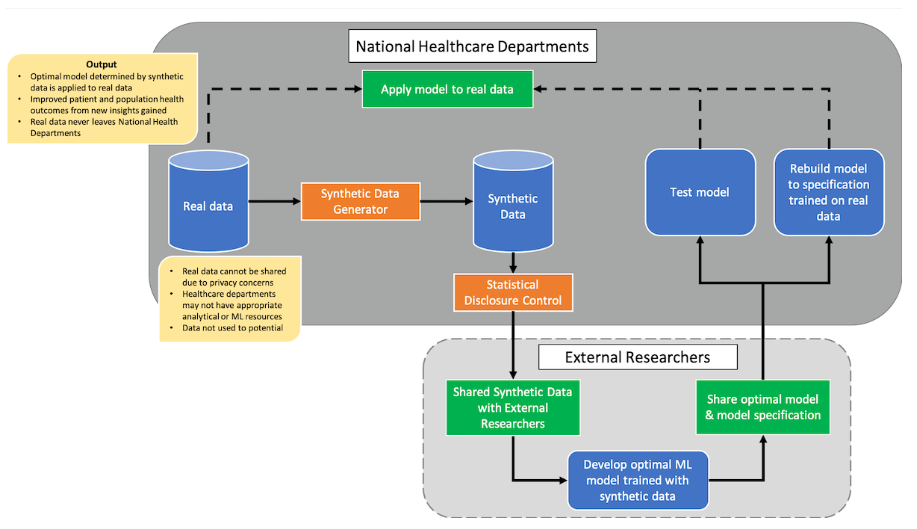
\includegraphics{assets/rankin.png}
    \caption{Distribution model for analysis.}
    \label{fig:open-data}
\end{figure}